% ─────────────────────────────────────────────────────────────────────────────
% Sec. 3  Background and Motivation. Prelim moved from the method section. Numbers in 3.2 and the figure / tables are
% generated by paper/figures/make_recall_figure.py (post-hoc analysis of frozen v1.0 on V* Bench); 3.1 quotes tab_hr8k.
% ─────────────────────────────────────────────────────────────────────────────
\section{Background and Motivation}
\label{sec:motivation}

% ─────────────────────────────────────────────────────────────────────────────
\subsection{Where the cost of high resolution comes from}
\label{sec:prelim}

We build on dynamic-resolution VLMs~\cite{internvl15}, using InternVL3.5~\cite{internvl35} as the running
example. An image is resized to a grid of $c\times r$ tiles of $448\times448$ pixels whose aspect ratio is
closest to that of the image, with $N=cr\le N_{\max}$, and a global thumbnail is appended when $N>1$. Each
tile is encoded independently and turned into $n=256$ visual tokens by pixel shuffle and an MLP projector.
\method relies on this independence, which other tile-based VLMs such as LLaVA-OneVision~\cite{llavaov}
share. The language model then prefills $[\,\mathbf{x}_b;\ \mathbf{V}_1;\ \dots;\ \mathbf{V}_{N+1};\
\mathbf{x}_a\,]$, where $\mathbf{x}_b$ is the text before the image, $\mathbf{V}_t\in\mathbb{R}^{n\times d}$
are the tokens of tile $t$, and $\mathbf{x}_a$ is the question with the answer prefix. Vision-encoder
compute, prefill, and the KV cache all grow with $N$, the attention of prefill even as $\mathcal{O}(N^2)$.
With $N_{\max}=47$, a 4K image already yields 24 to 45 tiles; without a cap, an 8K image yields 188 tiles
(48K visual tokens).

Token pruning removes tokens \emph{after} they are computed: VisionZip~\cite{visionzip} and
HiRED~\cite{hired} after the vision encoder, which still sees all $N$ tiles, and FastV~\cite{fastv},
SparseVLM~\cite{sparsevlm}, and IF-Prune~\cite{ifprune} inside the language model, whose first layers still
process all $nN$ tokens. On HR-Bench 8K with 188 tiles and $B=1536$, the latter keep only 3.2\% of the 48K
visual tokens, yet need more than 8\,GB of memory and 3.2 to 7.0\,s to the first token, and VisionZip and
HiRED still encode all 188 tiles (\cref{tab:hr8k}). Cost follows the input, not what is kept.

% ─────────────────────────────────────────────────────────────────────────────
\subsection{How reliable is low-resolution attention}
\label{sec:reliability}

Encoding only a few tiles means choosing them from a view in which the target may not even be resolved: on
V$^*$~Bench~\cite{vstar}, 80\% of the target objects are smaller than one ViT patch in the thumbnail. We
measure this choice on V$^*$~Bench, the only one of our benchmarks with target boxes, and count a hit if at
least half of the box of each target lies in the chosen tiles. We analyze the two signals of the frozen
method (\cref{sec:impl}): the coarse prior, \ie the attention that the question pays to a low-resolution view
(\cref{sec:prior}), and boundary scoring, which re-scores a few tiles near the cut-off with their
high-resolution tokens (\cref{sec:boundary}). No parameter was chosen from this analysis.

\begin{figure}[t]
  \centering
  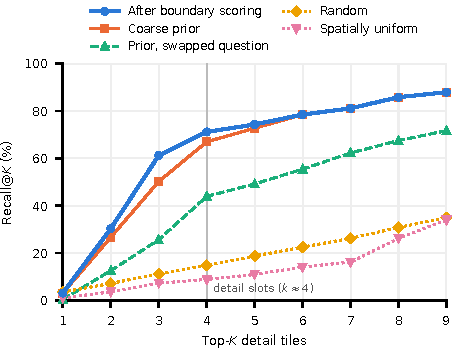
\includegraphics[width=\linewidth]{figures/fig_recall.pdf}
  \caption{\textbf{Reliability of low-resolution attention} on V$^*$~Bench ($B=1536$). Recall@$K$ is the
  fraction of questions whose target is covered by the top $K$ detail tiles. Swapped question: the prior
  computed with the question of another image of the same category.}
  \label{fig:recall}
\end{figure}

\paragraph{The prior can filter.}
With the top four of a median of 24 tiles, the coarse prior covers the target on 67.0\% of the questions, against
14.8\% for random and 8.9\% for spatially uniform selection (\cref{fig:recall}). It also follows the question:
with the question of another image, recall drops to 44.0\%, by 23.0 points (95\% CI [15.7, 30.9]).

\paragraph{The decision needs high resolution.}
The first-ranked tile of the prior covers the target on only 3.1\% of the questions. At the same $K$, boundary
scoring raises recall at every budget, from 27.7\% to 69.1\% at $B=1024$ and from 67.0\% to 71.2\% at
$B=1536$, and it recovers 64 to 90\% of the targets in the window that the prior alone would miss
(\cref{tab:recall,tab:window}). This recall is not the final accuracy, which \cref{sec:main} reports.

% ─────────────────────────────────────────────────────────────────────────────
\subsection{Motivation}
\label{sec:design}

These observations motivate three design choices of \method: since cost arises when tiles are computed, the
decision is made before the vision encoder and the KV cache is built by streaming; since low-resolution
attention finds candidates for the question, the VLM's own attention over a low-resolution view filters the
tiles, without any other model; and since the final choice needs high resolution only near the cut-off, only
a small boundary window is encoded and scored.

\paragraph{Problem setting.}
Given a budget of $B$ visual tokens, \ie $K=\lfloor B/n\rfloor$ tiles, we want to choose \emph{before
encoding} which tiles to keep, such that the vision encoder, the language model, and the KV cache
each process $\mathcal{O}(K)$ tokens independently of $N$.
